\section{Supplementary Materials}


\begin{figure}[H]

{\centering \pandocbounded{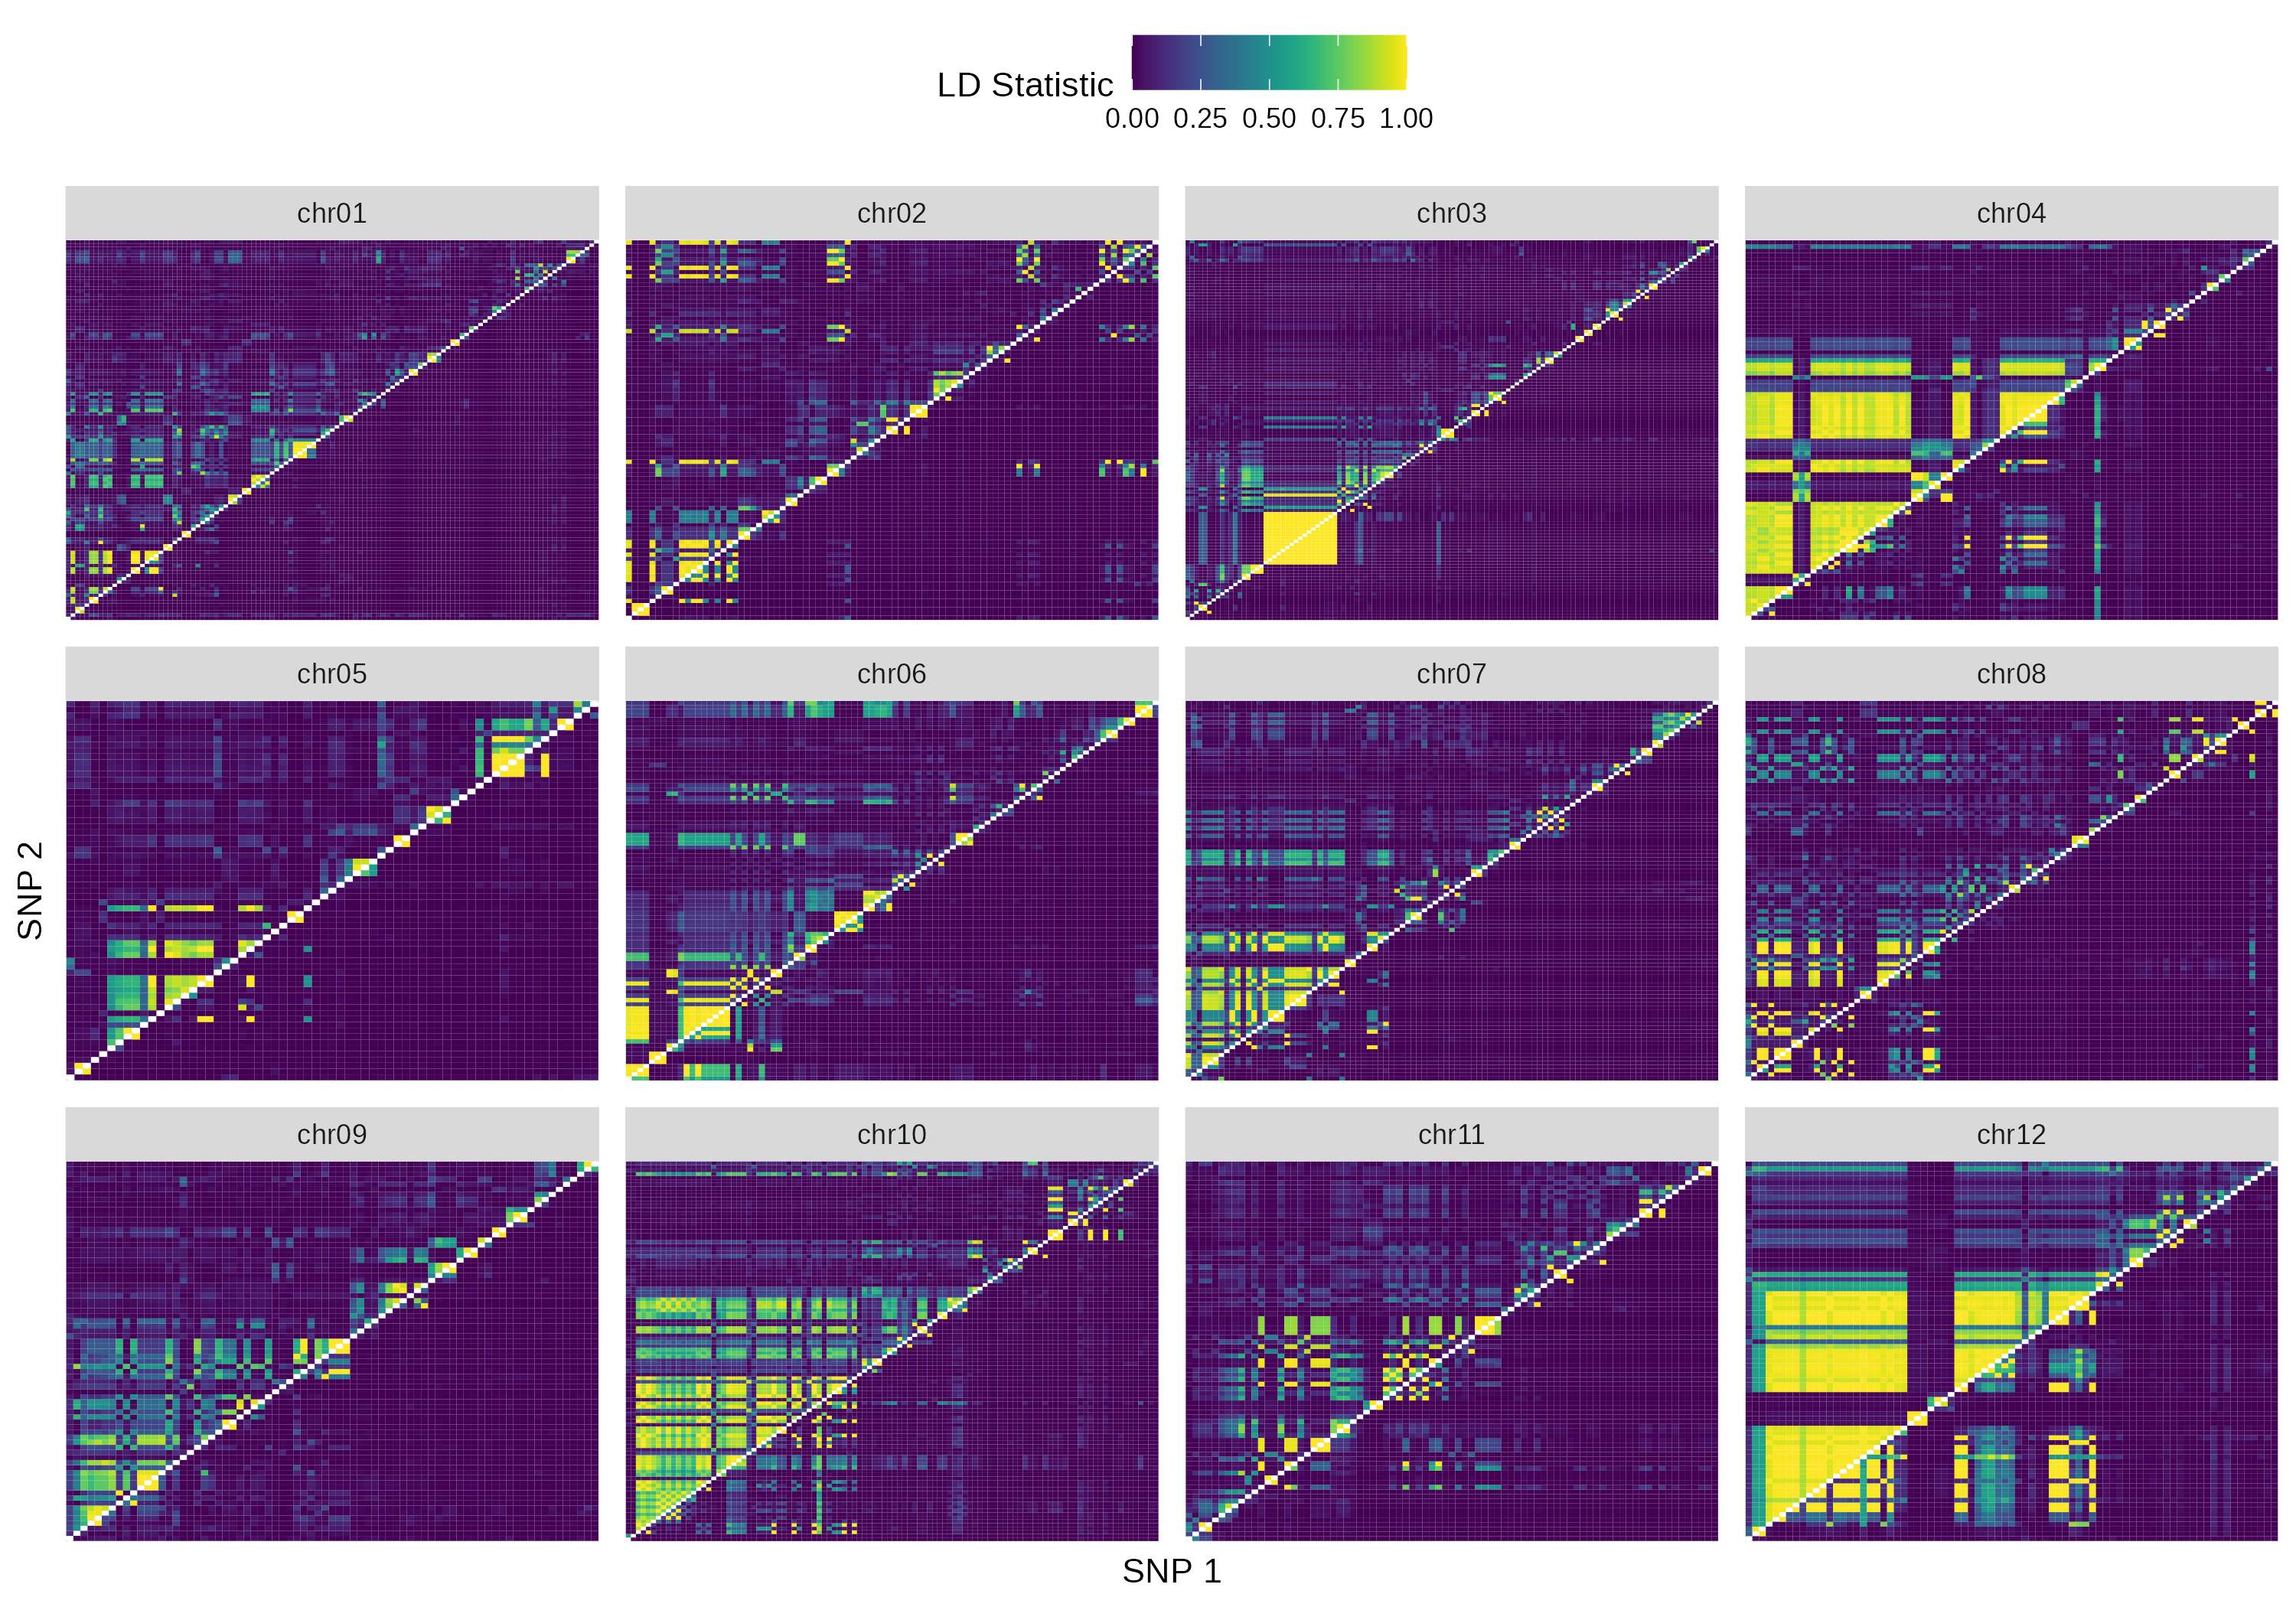
\includegraphics[keepaspectratio]{figs_03/1664221645_LD_Estimates.png}}

}

\caption{Estimates of within-chromosome linkage disequilibrium per 12
chromosomes. Above the diagonal is the conventional r\textsuperscript{2}
statistic and below the diagonal is the
r\textsuperscript{2}\textsubscript{v} statistic resolved for population
history.}

\end{figure}%

\begin{table}

\caption{Summary of Polymorphism Information Content (PIC) and proportion of marker homozygosity per chromosome}
\centering
\begin{tabular}[t]{lrrrrrr}
\toprule
\multicolumn{1}{c}{} & \multicolumn{2}{c}{Average PIC} & \multicolumn{2}{c}{Average Proportion Homozygosity} & \multicolumn{2}{c}{Number of Probes} \\
\cmidrule(l{3pt}r{3pt}){2-3} \cmidrule(l{3pt}r{3pt}){4-5} \cmidrule(l{3pt}r{3pt}){6-7}
Chromosome & LD Filter & Unfiltered & LD Filter & Unfiltered & LD Filter & Unfiltered\\
\midrule
chr01 & 0.279 & 0.275 & 0.849 & 0.853 & 92 & 115\\
chr02 & 0.277 & 0.268 & 0.854 & 0.860 & 56 & 90\\
chr03 & 0.281 & 0.274 & 0.850 & 0.851 & 81 & 123\\
chr04 & 0.267 & 0.271 & 0.875 & 0.875 & 53 & 90\\
chr05 & 0.259 & 0.262 & 0.885 & 0.883 & 45 & 65\\
\addlinespace
chr06 & 0.302 & 0.295 & 0.857 & 0.865 & 52 & 92\\
chr07 & 0.297 & 0.305 & 0.869 & 0.866 & 66 & 97\\
chr08 & 0.275 & 0.260 & 0.870 & 0.876 & 58 & 93\\
chr09 & 0.253 & 0.250 & 0.887 & 0.885 & 57 & 75\\
chr10 & 0.291 & 0.289 & 0.845 & 0.824 & 52 & 106\\
\addlinespace
chr11 & 0.288 & 0.271 & 0.866 & 0.873 & 53 & 81\\
chr12 & 0.290 & 0.312 & 0.874 & 0.866 & 39 & 79\\
Whole-Genome & 0.280 & 0.278 & 0.865 & 0.865 & 704 & 1106\\
\bottomrule
\end{tabular}
\end{table}

\begin{figure}[H]

{\centering \pandocbounded{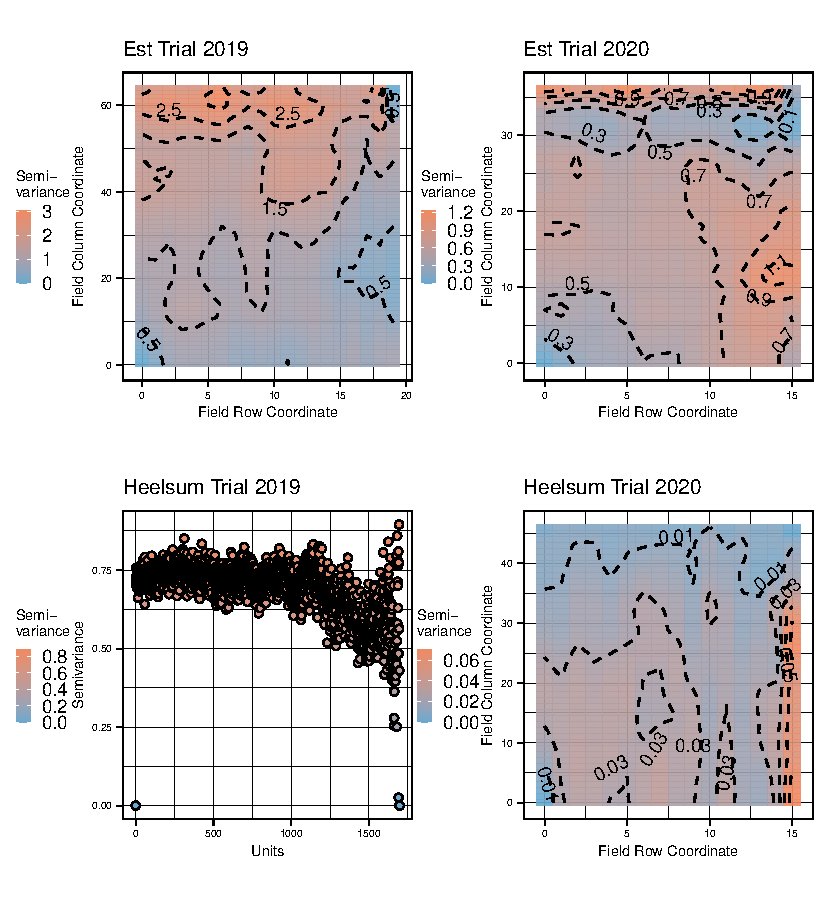
\includegraphics[keepaspectratio]{figs_03/vario-dm-1.pdf}}

}

\caption{Emperical variograms on row and column coordinates for
percentage of tuber dry matter content in Est and Heelsum field trials
in 2019 and 2020. Because both trials in Heelsum were modelled with no
residual structures, the variogram is plotted only with respect to
observation.}

\end{figure}%

\begin{figure}[H]

{\centering \pandocbounded{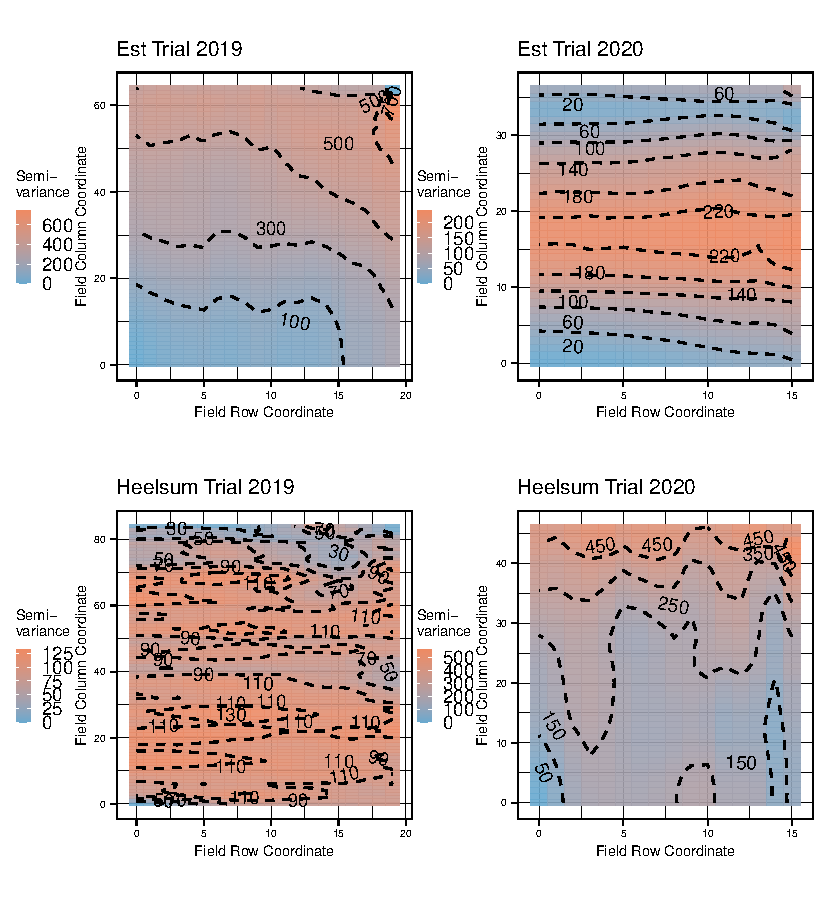
\includegraphics[keepaspectratio]{figs_03/vario-tn-1.pdf}}

}

\caption{Emperical variograms on row and column coordinates for total
tuber number in Est and Heelsum field trials in 2019 and 2020.}

\end{figure}%

\begin{figure}[H]

{\centering \pandocbounded{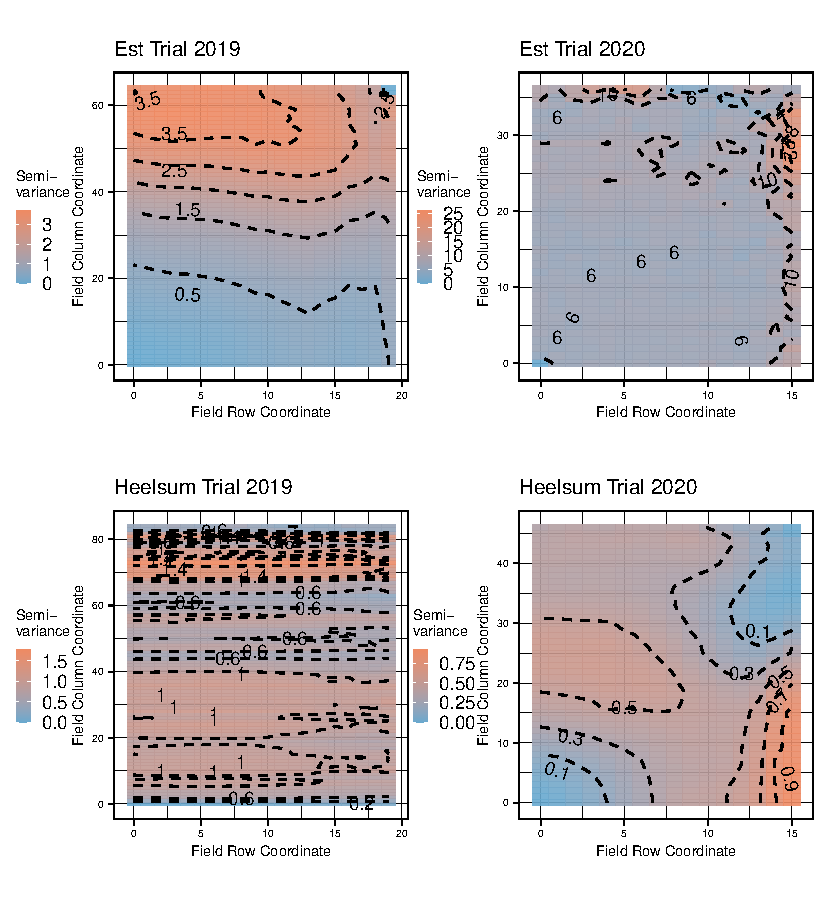
\includegraphics[keepaspectratio]{figs_03/vario-tv-1.pdf}}

}

\caption{Emperical variograms on row and column coordinates for average
tuber volume in Est and Heelsum field trials in 2019 and 2020. Because
the 2020 Heelsum trial was modelled wih no residual structure, the
variogram is plotted only with respect to observation.}

\end{figure}%

\begin{figure}[H]

{\centering \pandocbounded{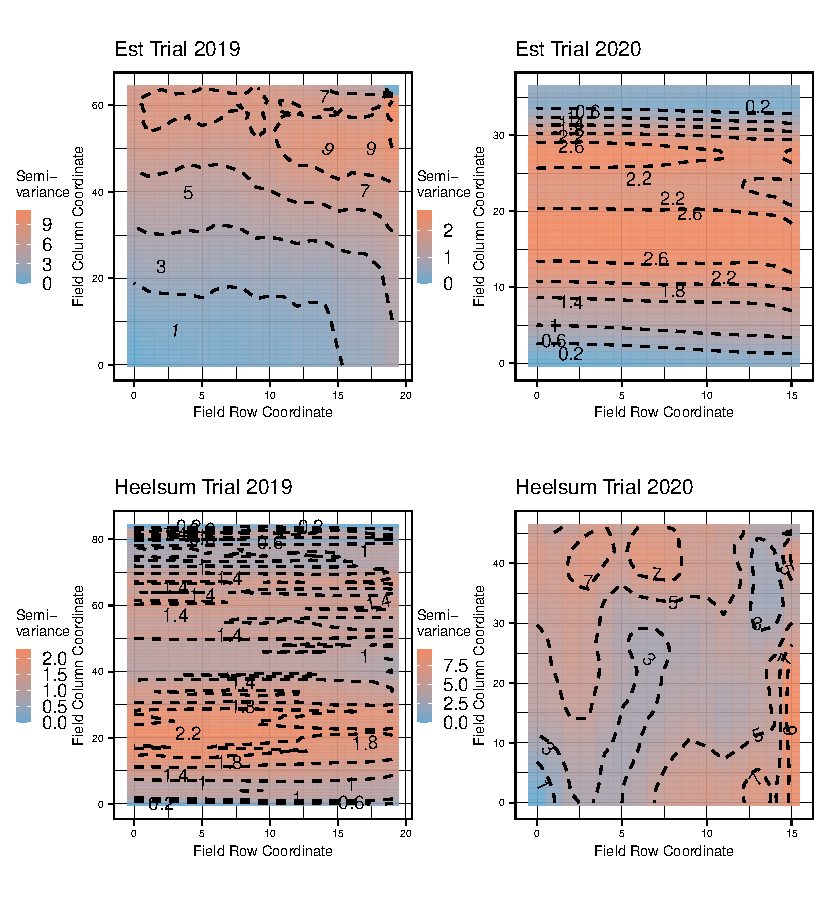
\includegraphics[keepaspectratio]{figs_03/vario-ty-1.pdf}}

}

\caption{Emperical variograms with respect to row and column coordinates
for total tuber yield in Est and Heelsum field trials in 2019 and 2020.}

\end{figure}%

\begin{table}
\caption{Median prediction accuracies and median coefficient of error (The root
mean square error scaled by phenotype mean) for each trait, test cross
scenario, and prediction target. This was conducted on dry matter
content (DM), total tuber number (TN), mean tuber volume (TV), and total
tuber yield (TY). Predictions were either compared to BLUE's generated
from the first stage of modelling for Est 2019 and 2020 (E19 and E20,
repsectively) and Heelsum 2019 and 2022 (H19 and H20, respectively) or
against across-trial BLUP's (BLP) produced from model @eq-multi-pheno.}\tabularnewline

\centering
\resizebox{\linewidth}{!}{
\begin{tabular}{lllll}
\toprule
\multicolumn{1}{c}{} & \multicolumn{2}{c}{0 Common Parent Set} & \multicolumn{2}{c}{1 Common Parent Set} \\
\cmidrule(l{3pt}r{3pt}){2-3} \cmidrule(l{3pt}r{3pt}){4-5}
Trail Target & GCA & GCA+SCA & GCA & GCA+SCA\\
\midrule
\addlinespace[0.3em]
\multicolumn{5}{l}{\textbf{DM}}\\
\hspace{1em}E19 & 0.45 (12.5) & 0.45 (12.4) & 0.54 (11.8) & 0.54 (11.8)\\
\hspace{1em}E20 & 0.57 (9.9) & 0.56 (9.9) & 0.63 (9.4) & 0.63 (9.4)\\
\hspace{1em}H19 & 0.40 (10.4) & 0.40 (10.3) & 0.49 (9.8) & 0.49 (9.8)\\
\hspace{1em}H20 & 0.52 (8.5) & 0.51 (8.5) & 0.63 (7.8) & 0.63 (7.8)\\
\hspace{1em}BLP & 0.49 (7.9) & 0.49 (7.9) & 0.58 (7.4) & 0.58 (7.4)\\
\addlinespace[0.3em]
\multicolumn{5}{l}{\textbf{TN}}\\
\hspace{1em}E19 & 0.36 (21.4) & 0.36 (21.4) & 0.45 (20.4) & 0.46 (20.3)\\
\hspace{1em}E20 & 0.26 (20.7) & 0.28 (20.7) & 0.39 (19.8) & 0.41 (19.7)\\
\hspace{1em}H19 & 0.39 (33.3) & 0.39 (33.3) & 0.51 (31.6) & 0.50 (31.5)\\
\hspace{1em}H20 & 0.32 (27.6) & 0.32 (27.6) & 0.47 (26.6) & 0.46 (26.7)\\
\hspace{1em}BLP & 0.36 (20.8) & 0.36 (20.7) & 0.50 (19.7) & 0.51 (19.6)\\
\addlinespace[0.3em]
\multicolumn{5}{l}{\textbf{TV}}\\
\hspace{1em}E19 & 0.54 (20.9) & 0.54 (20.8) & 0.61 (19.3) & 0.61 (19.2)\\
\hspace{1em}E20 & 0.70 (22.8) & 0.71 (22.7) & 0.73 (21.5) & 0.73 (21.4)\\
\hspace{1em}H19 & 0.57 (25.2) & 0.58 (25.2) & 0.65 (23.6) & 0.65 (23.5)\\
\hspace{1em}H20 & 0.62 (32.1) & 0.62 (32.2) & 0.68 (29.2) & 0.68 (29.2)\\
\hspace{1em}BLP & 0.61 (21.2) & 0.61 (21.1) & 0.68 (19.4) & 0.68 (19.3)\\
\addlinespace[0.3em]
\multicolumn{5}{l}{\textbf{TY}}\\
\hspace{1em}E19 & 0.47 (21.9) & 0.47 (21.9) & 0.57 (20.8) & 0.58 (20.8)\\
\hspace{1em}E20 & 0.37 (21.4) & 0.38 (21.5) & 0.49 (20.3) & 0.49 (20.4)\\
\hspace{1em}H19 & 0.47 (46.5) & 0.47 (46.5) & 0.60 (43.7) & 0.60 (43.6)\\
\hspace{1em}H20 & 0.39 (35.7) & 0.39 (35.7) & 0.53 (34.5) & 0.53 (34.4)\\
\hspace{1em}BLP & 0.46 (27.3) & 0.46 (27.3) & 0.58 (25.3) & 0.58 (25.3)\\
\bottomrule
\end{tabular}}
\end{table}
